%%%%%%%%%%%%%%%%%%%%%%
\section{Conclusion}
%
%%%%%%%%%%%%%%%%%%%%%%

%%\subsection{}

All in all, we are satisfied with this result. The combination of a neural network and a clustering technique resulted in a relatively good detection method. We can detect wind parks in the North Sea area, with only very few false positive polygons - which are dense clusters of boats. The model and clustering techniques performed extremely well in the Skaggerak area, in stark contrast with the result in Chinese waters, where our model performs very poorly. Possibly due to the different orientation of the windmills, but further research is needed to know more about this issue.


\begin{figure}[ht]
\begin{center}
\centerline{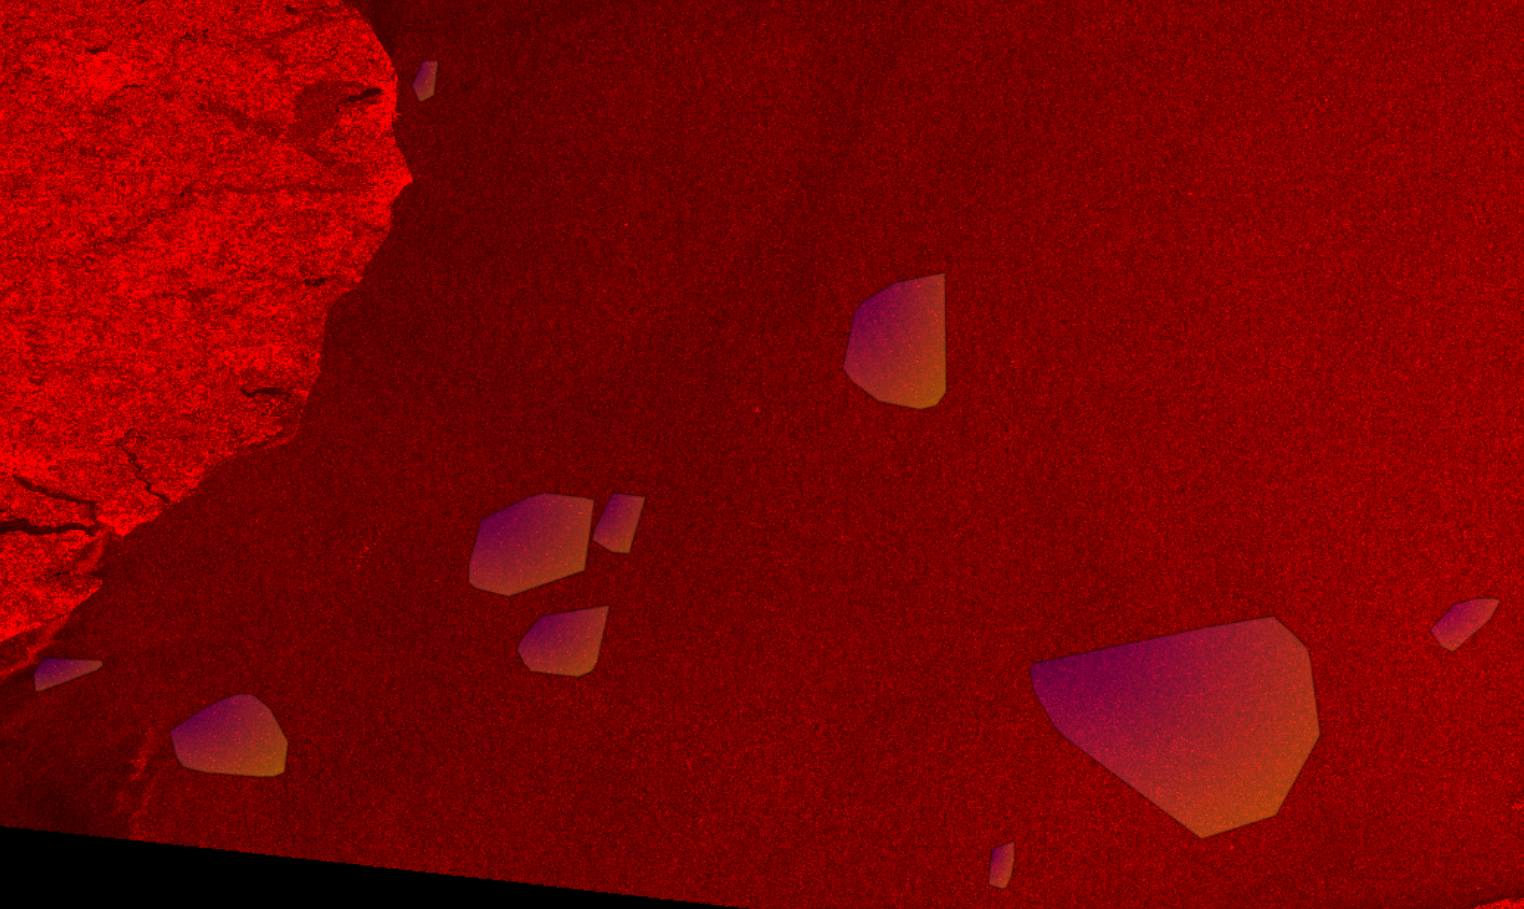
\includegraphics[width=\columnwidth]{images/result_northsea.png}}
\caption{Result North Sea area.}
\label{noise-reduction}
\end{center}
\end{figure}

\subsection{Future Work}
In order to distinguish boats from windmills we might think of using the same pictures with another timestamp. Moving objects are most likely boats and we expect to have a much better final result, however the computation load will increase. Using Sentinel's API in order to download new images automatically in order to set up a fully automated system might be something to consider for achieving a state-of-the-art way of identifying windmill parks.
